% !TEX root = ../om_ts_01.tex

\begin{frame} % frame name
	
	\videotitle{Data and Tasks}
	
\end{frame}



\begin{frame}{Data and Tasks: Plan}
	\begin{itemize}[<+->]
		\item Time series is a data type
		\item Tasks for one row
		\item Tasks for multiple rows
	\end{itemize}
	
\end{frame}





\begin{frame}{What is a time series?}
	
	\begin{block}{Time series}
		A sequence of observations ordered in time
		\[
		0, 0, 5, 7, 102, 53, 23
		\]
	\end{block}
	
	\pause
	\begin{block}{Time series}
		A sequence of random variables ordered in time
		\[
		y_1, y_2, y_3, y_4, \ldots, y_T
		\]
	\end{block}
	
	
\end{frame}


\begin{frame}{Tasks for one series}
	
	\begin{itemize}[<+->]
		\item Predict the following values
		\item Restore missing values in the middle of a series
		\item Restore individual observations from aggregated ones
		\item Detect point of discord (or structural break)
		\item Decompose series to a trend and seasonal parts
		\item \ldots
	\end{itemize}
	
\end{frame}


\begin{frame}{Forecasting}
	
	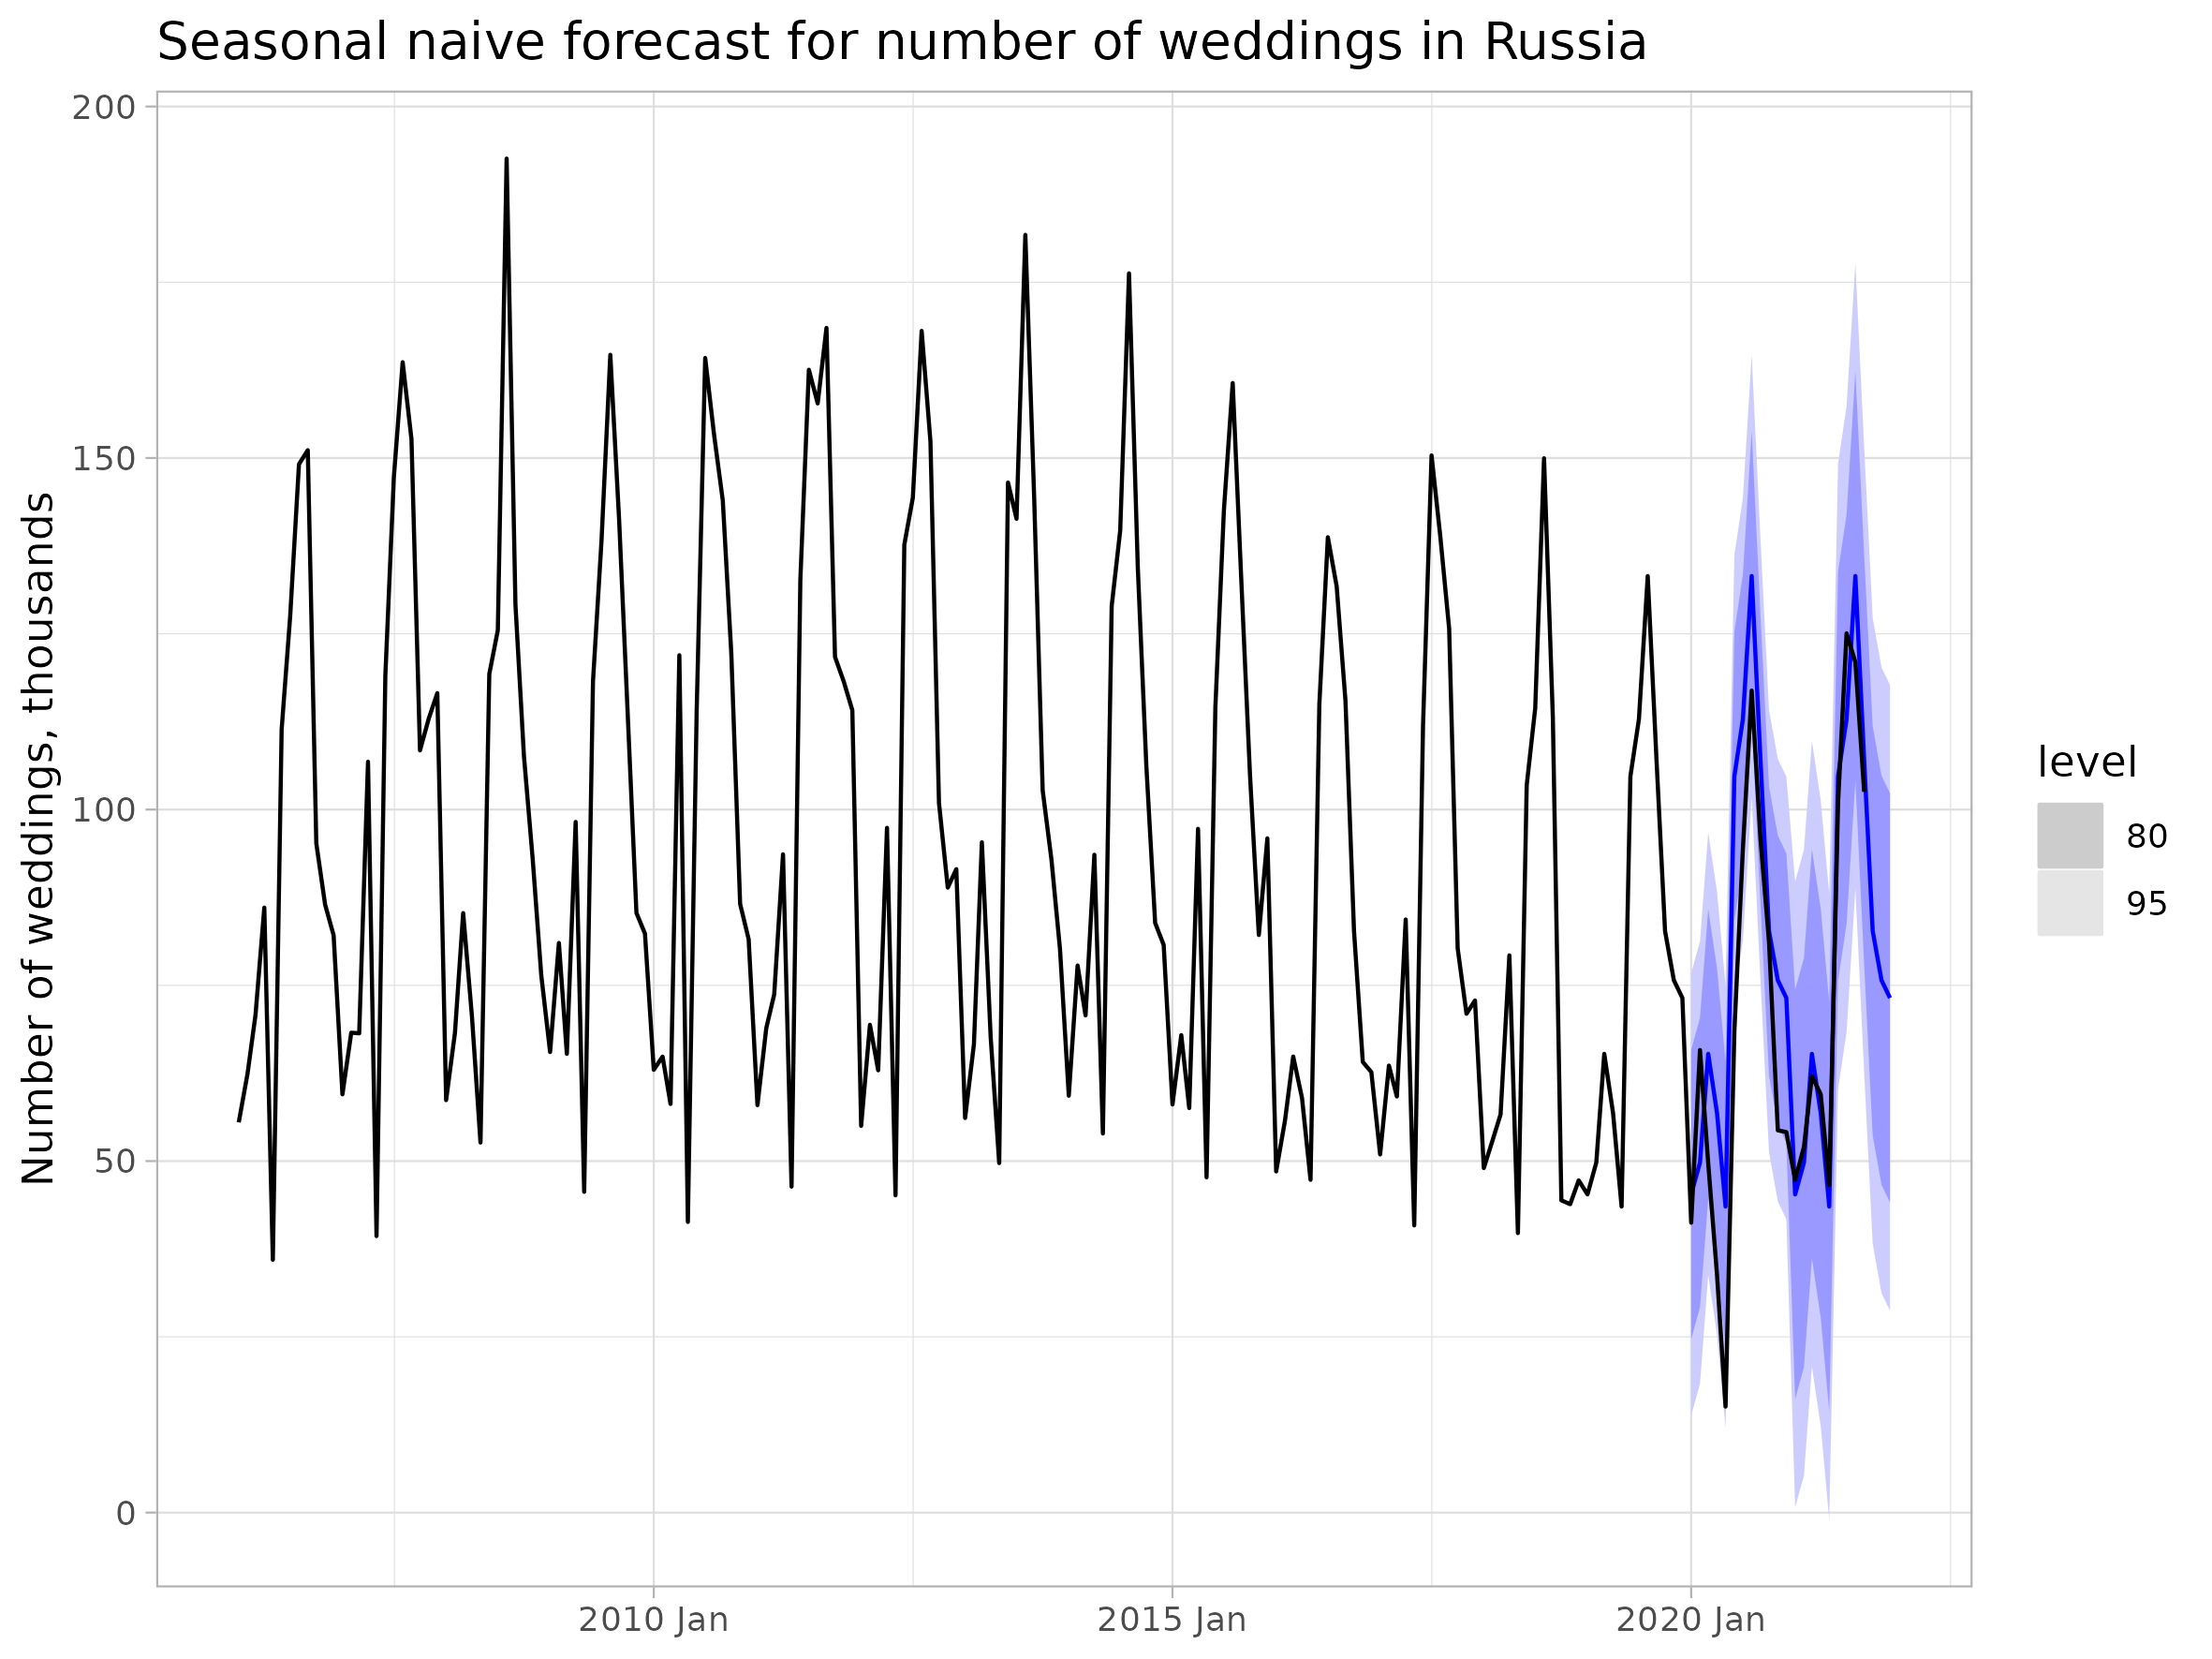
\includegraphics[width=\textwidth]{pictures/om_ts_01-017.png}
	
\end{frame}


\begin{frame}{Tasks for multiple series}
	
	\begin{itemize}[<+->]
		\item Use additional series when studying the target series
		\item Understand if series are related
		\item Measure cause and effect relationships
		\item Classify the new series into one of the existing classes
		\item Understand which series are close to each other
		\item Cluster series into an unknown set of clusters
		\item \ldots
	\end{itemize}
	
\end{frame}

\begin{frame}{Measuring series proximity}
	
	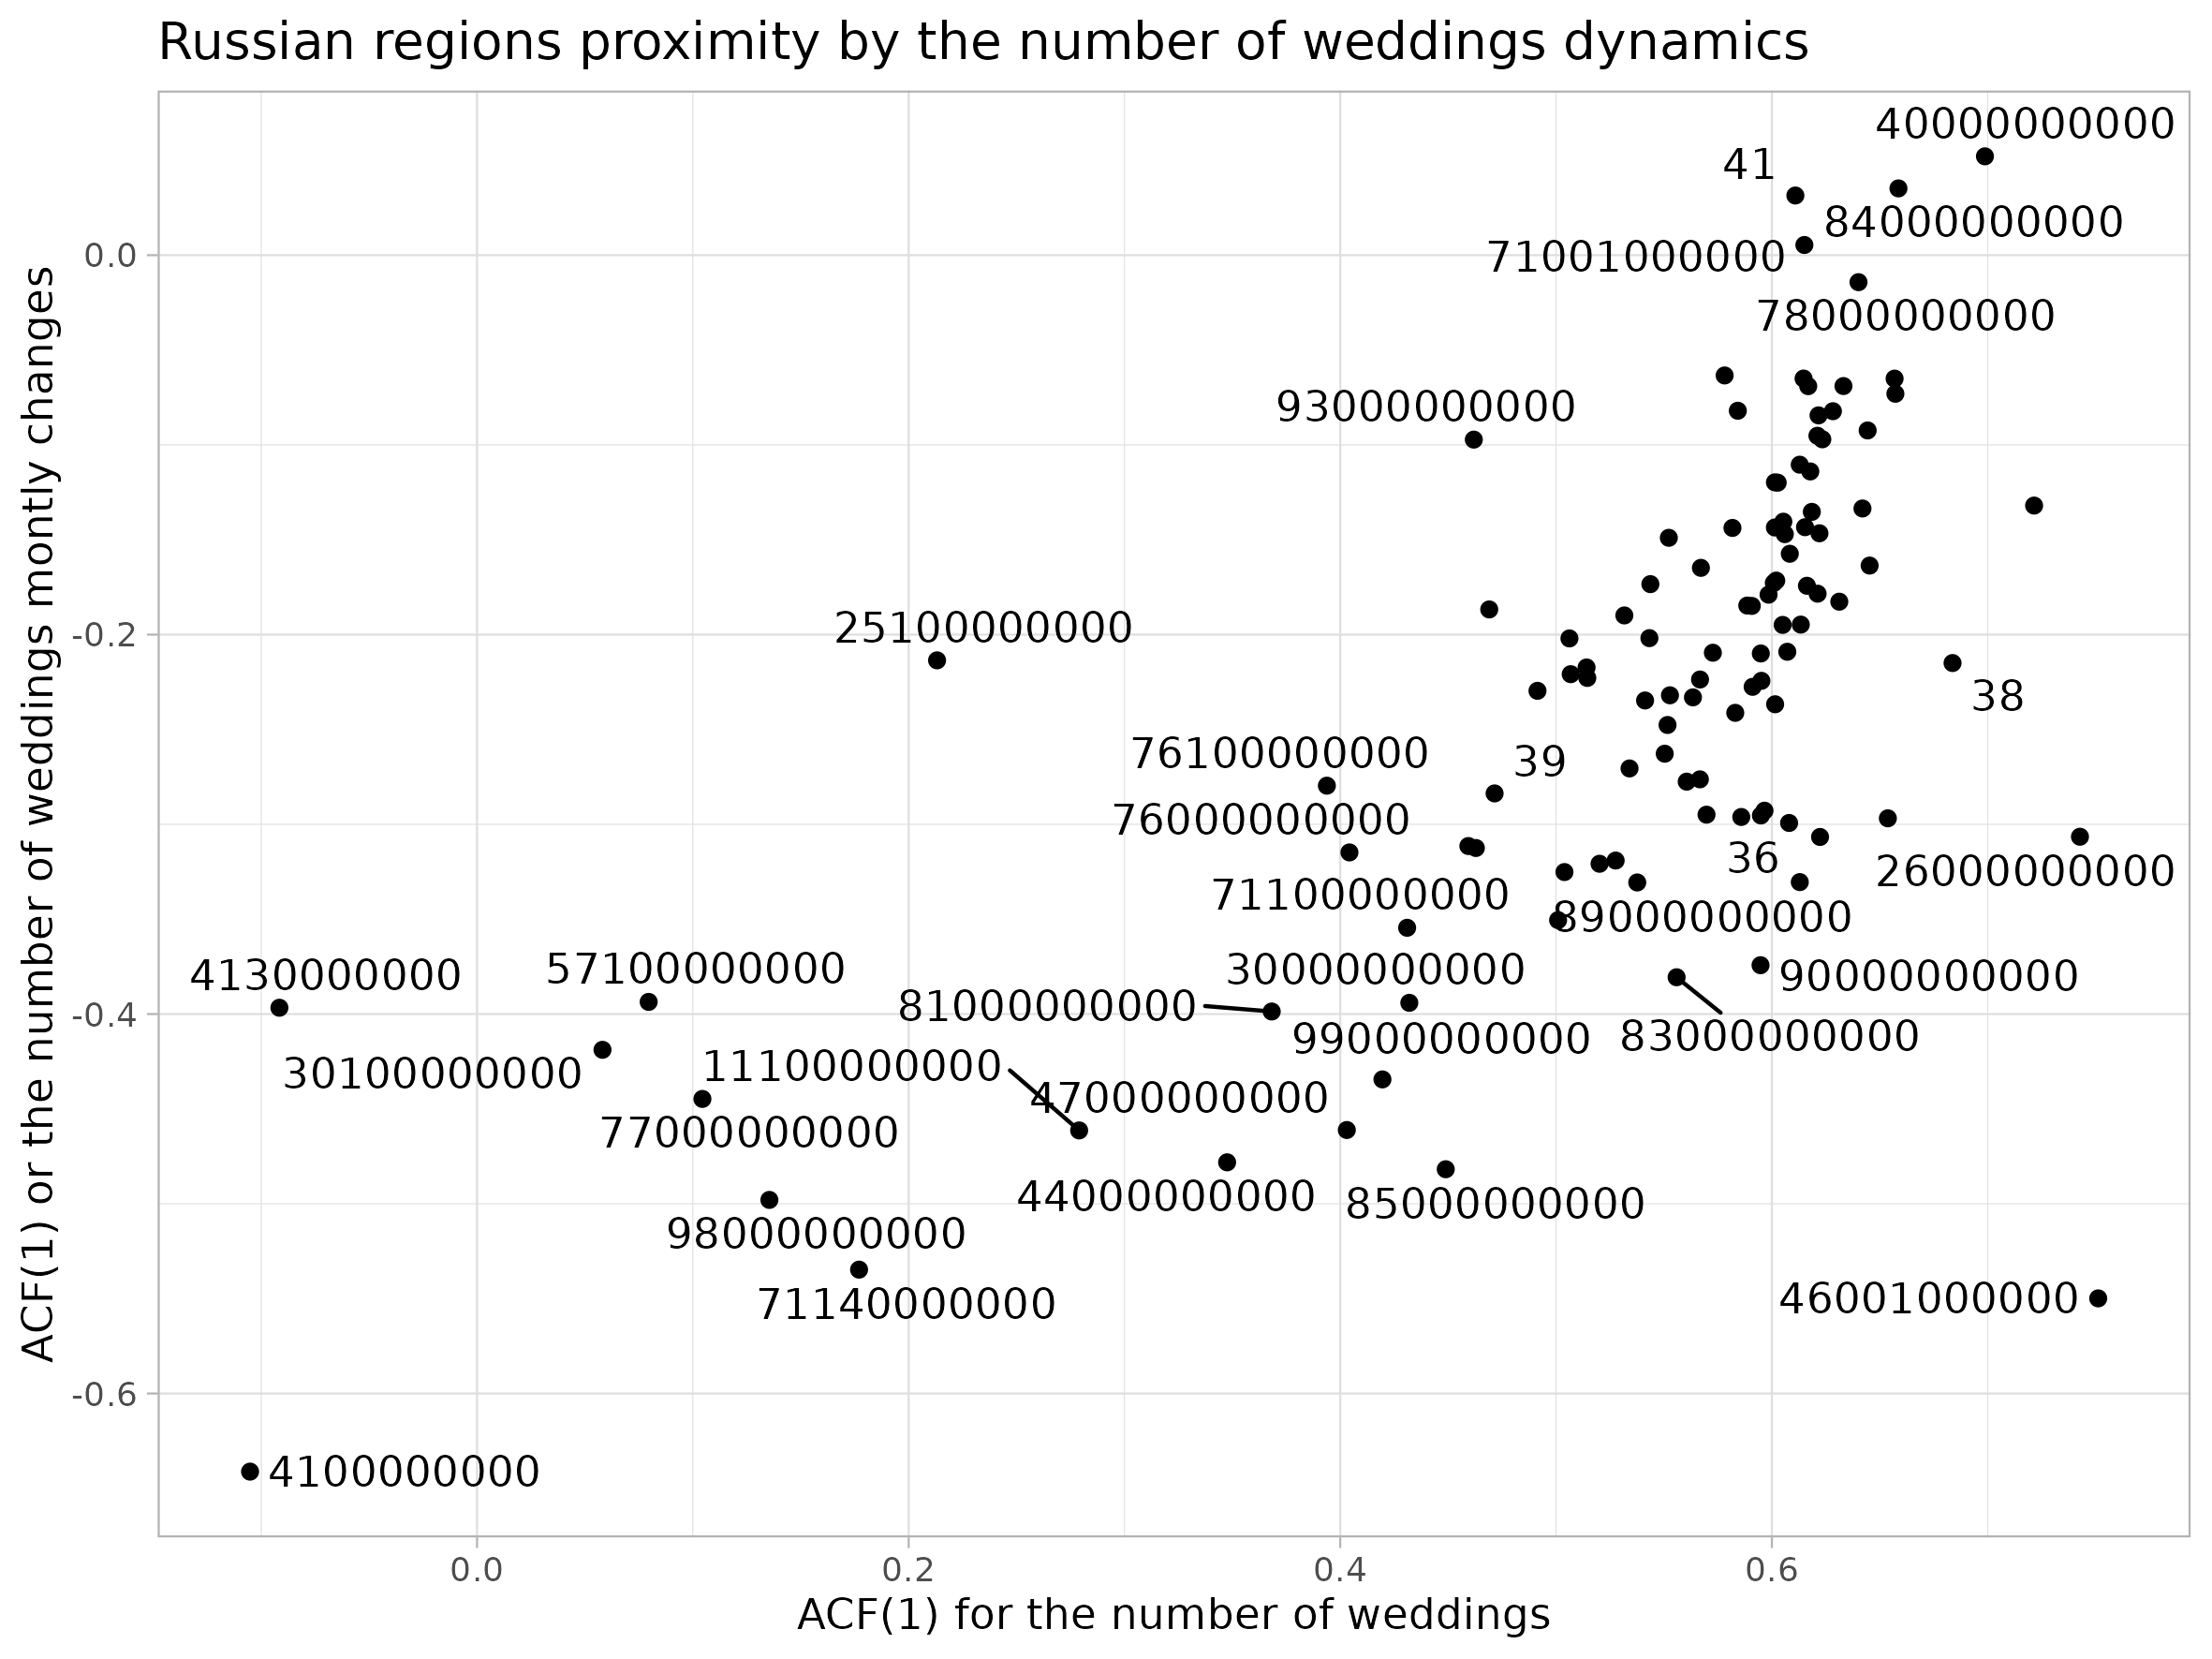
\includegraphics[width=\textwidth]{pictures/om_ts_01-025.png}
	
	
\end{frame}



\begin{frame}{Models and algorithms}
	
	\begin{block}{Models}
		\begin{itemize}[<+->]
			\item Explicit assumptions about the values $y_1$, $y_2$, \ldots, $y_T$
			\item Estimation method: maximum likelihood, Bayesian approach
			\item Point and interval forecasts, hypothesis testing
		\end{itemize}
	\end{block}
	
	ETS, ARIMA, ORBIT, PROPHET, \ldots
	
\end{frame}

\begin{frame}{Models and algorithms}
	
	\begin{block}{Algorithms}
		\begin{itemize}[<+->]
			\item Fuzzy assumptions about the values $y_1$, $y_2$, \ldots, $y_T$
			\item A special instruction for actions
			\item Point estimates without confidence intervals
		\end{itemize}
	\end{block}
	
	STL, gradient boosting, random forest, \ldots
	
\end{frame}

\begin{frame}{Course Focus}
	
	Forecasting one-dimensional series using models
	
\end{frame}